% Figure 1, panel B artwork only.  The panel identifier and caption belong in LaTeX.
\definecolor{ink}{HTML}{1F2937}
\definecolor{muted}{HTML}{64748B}
\definecolor{rulegray}{HTML}{CBD5E1}
\definecolor{calblue}{HTML}{2563A6}
\definecolor{deploygreen}{HTML}{2E7D5B}

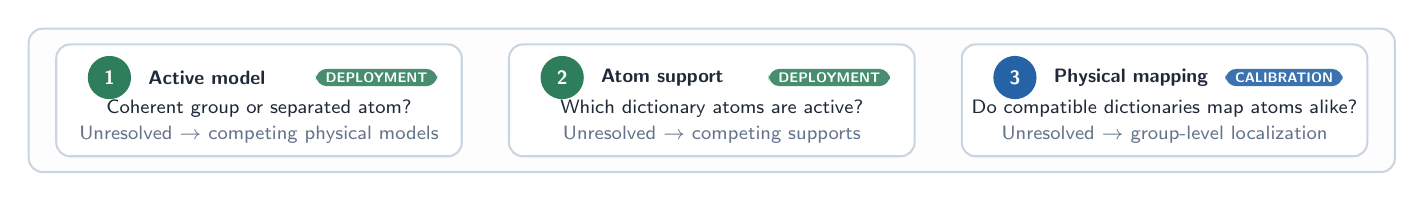
\begin{tikzpicture}[
  x=1cm,
  y=1cm,
  font=\sffamily,
  card/.style={draw=rulegray,line width=.75pt,rounded corners=5pt,fill=white},
  minipill/.style={rounded corners=4pt,inner xsep=3.5pt,inner ysep=1.4pt,
    font=\sffamily\bfseries\tiny,text=white},
  checkcard/.style={card,minimum width=5.15cm,minimum height=1.42cm}
]

% The three numbered questions are scientific content, not subfigure IDs.
\node[card,minimum width=17.35cm,minimum height=1.82cm,fill=ink!1]
  at (8.75,1.26) {};

\node[checkcard] at (3.00,1.26) {};
\node[circle,fill=deploygreen,text=white,font=\sffamily\bfseries\scriptsize,
  minimum size=.50cm] at (1.10,1.55) {1};
\node[font=\sffamily\bfseries\scriptsize,text=ink,anchor=west]
  at (1.47,1.55) {Active model};
\node[minipill,fill=deploygreen!88,anchor=east] at (5.27,1.55) {DEPLOYMENT};
\node[font=\sffamily\scriptsize,text=ink,align=center]
  at (3.00,1.15) {Coherent group or separated atom?};
\node[font=\sffamily\scriptsize,text=muted,align=center]
  at (3.00,.82) {Unresolved $\rightarrow$ competing physical models};

\node[checkcard] at (8.75,1.26) {};
\node[circle,fill=deploygreen,text=white,font=\sffamily\bfseries\scriptsize,
  minimum size=.50cm] at (6.85,1.55) {2};
\node[font=\sffamily\bfseries\scriptsize,text=ink,anchor=west]
  at (7.22,1.55) {Atom support};
\node[minipill,fill=deploygreen!88,anchor=east] at (11.02,1.55) {DEPLOYMENT};
\node[font=\sffamily\scriptsize,text=ink,align=center]
  at (8.75,1.15) {Which dictionary atoms are active?};
\node[font=\sffamily\scriptsize,text=muted,align=center]
  at (8.75,.82) {Unresolved $\rightarrow$ competing supports};

\node[checkcard] at (14.50,1.26) {};
\node[circle,fill=calblue,text=white,font=\sffamily\bfseries\scriptsize,
  minimum size=.50cm] at (12.60,1.55) {3};
\node[font=\sffamily\bfseries\scriptsize,text=ink,anchor=west]
  at (12.97,1.55) {Physical mapping};
\node[minipill,fill=calblue!90,anchor=east] at (16.77,1.55) {CALIBRATION};
\node[font=\sffamily\scriptsize,text=ink,align=center]
  at (14.50,1.15) {Do compatible dictionaries map atoms alike?};
\node[font=\sffamily\scriptsize,text=muted,align=center]
  at (14.50,.82) {Unresolved $\rightarrow$ group-level localization};
\end{tikzpicture}

